\documentclass{article}
\usepackage[utf8]{inputenc}
\usepackage{import}
\usepackage[subpreambles=true]{standalone}
\usepackage{graphicx}
\usepackage{amsmath}
\usepackage{amsfonts}
\usepackage{amssymb}
\usepackage{mathrsfs}
\usepackage{enumerate}
\usepackage{fancyhdr}
\usepackage[colorlinks=true,linkcolor=black,anchorcolor=black,citecolor=black,filecolor=black,menucolor=black,runcolor=black,urlcolor=blue]{hyperref}
\usepackage[margin=1.75in]{geometry}
\usepackage{algorithm, algpseudocode}
\usepackage{tikz-qtree}
\usepackage{ulem}

\tikzstyle{arr}=[fill=white, draw=black, shape=rectangle, scale=.85]
\tikzstyle{cir}=[fill=white, draw=black, shape=circle]

\begin{document}
%%%%%%%%%%%%%%%%%%%%%%%%%%%%
%%     Chapter Content    %%
%%%%%%%%%%%%%%%%%%%%%%%%%%%%
\section{Merge Sort}
\rule{\textwidth}{1pt}\\
\subsection{Pseudocode}
\begin{algorithm}
\caption{Merge Sort}
\begin{algorithmic}[1]
\Procedure{mergesort}{$A, p, r$}
	\If{$p<r$}
		\State $q\leftarrow \lfloor(p+r)/2\rfloor$
		\State \Call{mergesort}{$A, p, q$}
		\State \Call{mergesort}{$A, q+1, r$}
		\State \Call{merge}{$A, (p,q), (q+1,r)$}
	\EndIf
\EndProcedure
\Statex
\Procedure{merge}{$A, (p,q), (q+1,r)$}
	\State copy $(A, p, r)$ into $(B, p, r)$
	\State $i\leftarrow p$
	\State $j\leftarrow q+1$
	\State $k\leftarrow p$
	\While{$i\leq q$ and $j\leq r$}
		\If{$B[i] \leq B[j]$}
			\State $A[k]\leftarrow B[i]$
			\State $i\leftarrow i+1$
		\Else
			\State $A[k]\leftarrow B[j]$
			\State $j\leftarrow j+1$
		\EndIf
		\State $k\leftarrow k+1$
	\EndWhile
	\If{$i>q$}
		\State copy $(B, j, r)$ into $(A, k, r)$
	\Else
		\State copy $(B, i, q)$ into $(A, k, r)$
	\EndIf
\EndProcedure
\end{algorithmic}
\end{algorithm}

\subsection{Analysis of Merge}
\subsubsection*{Equal Size}
Best case, we only do $n$ comparisons (this is when $A_n < B_1$ or $B_n < A_1$).
Worst case is $2n-1$ comparisons (this is when $A_n$ and $B_n$ are the two largest elements).
The average case is $2n-2+\frac{2}{n+1}$.
\subsubsection*{Differing Sizes}
Let subarray $A$ be of size $m$ and subarray $B$ be of size $n$ where $m\leq n$.
Best case is $m$ comparisons (this is when $A_m < B_1$).
Worst case is $m+n-1$ (this is when $A_m$ and $B_n$ are the two largest elements).
When $m$ is much smaller than $n$ there are better algorithms we can use.
For $m=1$ binary search gives $\approx \lg n$.
\subsubsection*{Notes}
Merging is \textit{not} in place. It can be implemented in place but those 
algorithms are not practical.

\subsection{Analysis of Mergesort Comparisons}
We will analyze mergesort using the tree method, along with the assumption that $n$ is a 
power of $2$.
\begin{center}
	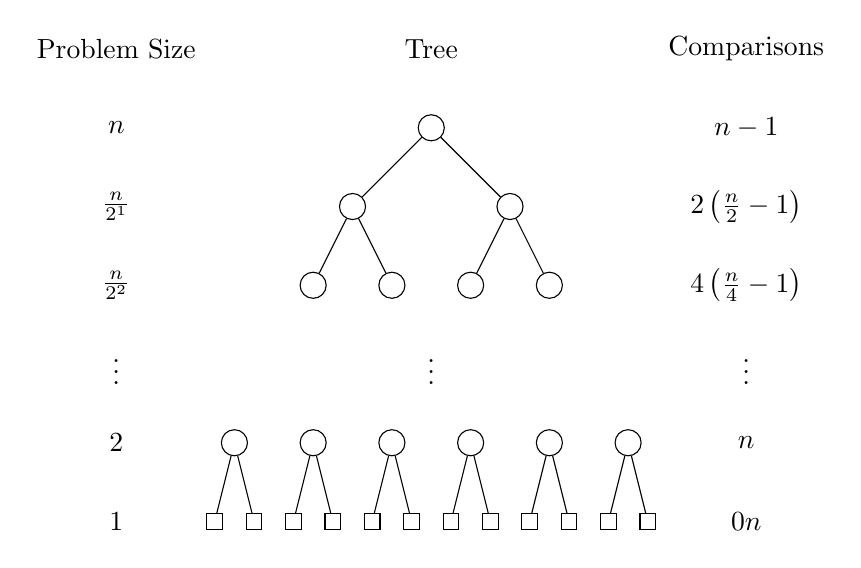
\begin{tikzpicture}
		\node (-10) at (-4, 1) {Problem Size};
		\node (-11) at (0, 1) {Tree};
		\node (-12) at (4, 1) {Comparisons};

		\node (10) at (-4, 0) {$n$};
		\node (11) at (-4, -1) {$\frac{n}{2^1}$};
		\node (12) at (-4, -2) {$\frac{n}{2^2}$};
		\node (13) at (-4, -3) {$\vdots$};
		\node (14) at (-4, -4) {$2$};
		\node (15) at (-4, -5) {$1$};

		\node (20) at (4, 0) {$n-1$};
		\node (21) at (4, -1) {$2\left(\frac{n}{2}-1\right)$};
		\node (22) at (4, -2) {$4\left(\frac{n}{4}-1\right)$};
		\node (23) at (4, -3) {$\vdots$};
		\node (24) at (4, -4) {$n$};
		\node (25) at (4, -5) {$0n$};

		\node [style=cir] (1) at (0,0) {};
		\node [style=cir] (2) at (-1,-1) {};
		\node [style=cir] (3) at (1,-1) {};
		\node [style=cir] (4) at (-1.5,-2) {};
		\node [style=cir] (5) at (-.5,-2) {};
		\node [style=cir] (6) at (.5,-2) {};
		\node [style=cir] (7) at (1.5,-2) {};

		\draw (2) to (1);
		\draw (3) to (1);
		\draw (4) to (2);
		\draw (5) to (2);
		\draw (6) to (3);
		\draw (7) to (3);

		\node (-1) at (0, -3) {$\vdots$};

		\node [style=cir] (31) at (-2.5, -4) {};
		\node [style=cir] (32) at (-1.5, -4) {};
		\node [style=cir] (33) at (-.5, -4) {};

		\node [style=cir] (41) at (2.5, -4) {};
		\node [style=cir] (42) at (1.5, -4) {};
		\node [style=cir] (43) at (.5, -4) {};

		\node [style=arr] (51) at (-2.75, -5) {};
		\node [style=arr] (52) at (-2.25, -5) {};
		\node [style=arr] (53) at (-1.75, -5) {};
		\node [style=arr] (54) at (-1.25, -5) {};
		\node [style=arr] (55) at (-.75, -5) {};
		\node [style=arr] (56) at (-.25, -5) {};

		\node [style=arr] (61) at (2.75, -5) {};
		\node [style=arr] (62) at (2.25, -5) {};
		\node [style=arr] (63) at (1.75, -5) {};
		\node [style=arr] (64) at (1.25, -5) {};
		\node [style=arr] (65) at (.75, -5) {};
		\node [style=arr] (66) at (.25, -5) {};

		\draw (51) to (31);
		\draw (52) to (31);
		\draw (53) to (32);
		\draw (54) to (32);
		\draw (55) to (33);
		\draw (56) to (33);

		\draw (61) to (41);
		\draw (62) to (41);
		\draw (63) to (42);
		\draw (64) to (42);
		\draw (65) to (43);
		\draw (66) to (43);
	\end{tikzpicture}
\end{center}
We can notice that each level does exactly $2^k (\frac{n}{2^k} -1)$ comparisons
where $k$ is the level of that branch, it follows then that since the height of the tree is
$\lg n$, the total number of comparisons is
\begin{align*}
	\sum_{i=0}^{\lg n-1} 2^i \left(\frac{n}{2^i} -1\right) &= \sum_{i=0}^{\lg n-1} \left(n-2^i\right) \\
	&= \sum_{i=0}^{\lg n-1}n - \sum_{i=0}^{\lg n-1} 2^i \\
	&= (n\lg n) - \left(2^{\lg n -1+1} -1\right) \\
	&= (n\lg n) - (n-1) \\
	&= n\lg n -n +1
\end{align*}
As a recurrence,
\begin{align*}
	T(n) &= T\left(\frac{n}{2}\right) + T\left(\frac{n}{2}\right) + (n-1) \\
	&= 2T\left(\frac{n}{2}\right) + n - 1, \hspace{3mm} T(0)=T(1)=0
\end{align*}


\end{document}